
This format seems to be the universally accepted format for 2D and 3D visualisation in 
Computational Geodynamics (and even CFD ?). Such files can be opened with open source 
softwares such as 
Paraview \footnote{https://www.paraview.org/}, 
MayaVi \footnote{https://docs.enthought.com/mayavi/mayavi/}
or Visit \footnote{https://wci.llnl.gov/simulation/computer-codes/visit/}.

Unfortunately it is my experience that no simple tutorial exists about how to build 
such files. There is an official document which describes the vtk 
format\footnote{https://www.vtk.org/wp-content/uploads/2015/04/file-formats.pdf}
but it delivers the information in a convoluted way. I therefore describe hereafter 
how \fieldstone{} builds the vtk files. 

I hereunder show vtk file corresponding to a 3x2 grid made of linear elements.
In this particular example there are:
\begin{itemize}
\item 12 nodes and 6 elements
\item 1 elemental field (the pressure {\tt p}
\item 2 nodal fields: 1 scalar (the smoothed pressure {\tt q}), 1 vector (the velocity field {\tt u,v,0})
\end{itemize}
Note that vtk files are inherently 3D so that even in the case of a 2D simulation the $z$-coordinate 
of the points and for instance their $z$-velocity component must be provided.
The file, usually called {\filenamefont solution.vtk} starts with a header:

\lstinputlisting[language=python,firstline=1,lastline=3]{images/vtk/solution.vtu}

We then proceed to write the node coordinates as follows:

\lstinputlisting[language=python,firstline=4,lastline=19]{images/vtk/solution.vtu}

These are followed by the elemental field(s):

\lstinputlisting[language=python,firstline=20,lastline=29]{images/vtk/solution.vtu}

Nodal quantities are written next:

\lstinputlisting[language=python,firstline=30,lastline=59]{images/vtk/solution.vtu}

To these informations we must append 3 more datasets. The first one is the connectivity, 
the second one is the offsets and the third one is the type. The first one is trivial
since the required connectivity array is the same as the one needed for the Finite Elements. 
The second must be understood as follows:
when reading the connectivity information in a linear manner the offset values 
indicate the beginning of each element (omitting the zero value). The third is simply the type of element 
as given in the vtk format document (9 corresponds to a generic quadrilateral with an 
internal numbering consistent with ours). 

\lstinputlisting[language=python,firstline=60,lastline=85]{images/vtk/solution.vtu}

The file is then closed with

\lstinputlisting[language=python,firstline=86,lastline=88]{images/vtk/solution.vtu}

The {\sl solution.vtu}\footnote{\url{https://raw.githubusercontent.com/cedrict/fieldstone/master/images/vtk/solution.vtu}}  
can then be opened with ParaView, MayaVi or Visit and the reader 
is advised to find tutorials online on how to install and use these softwares. Also check Appendix~\ref{app:paraview}.

\begin{center}
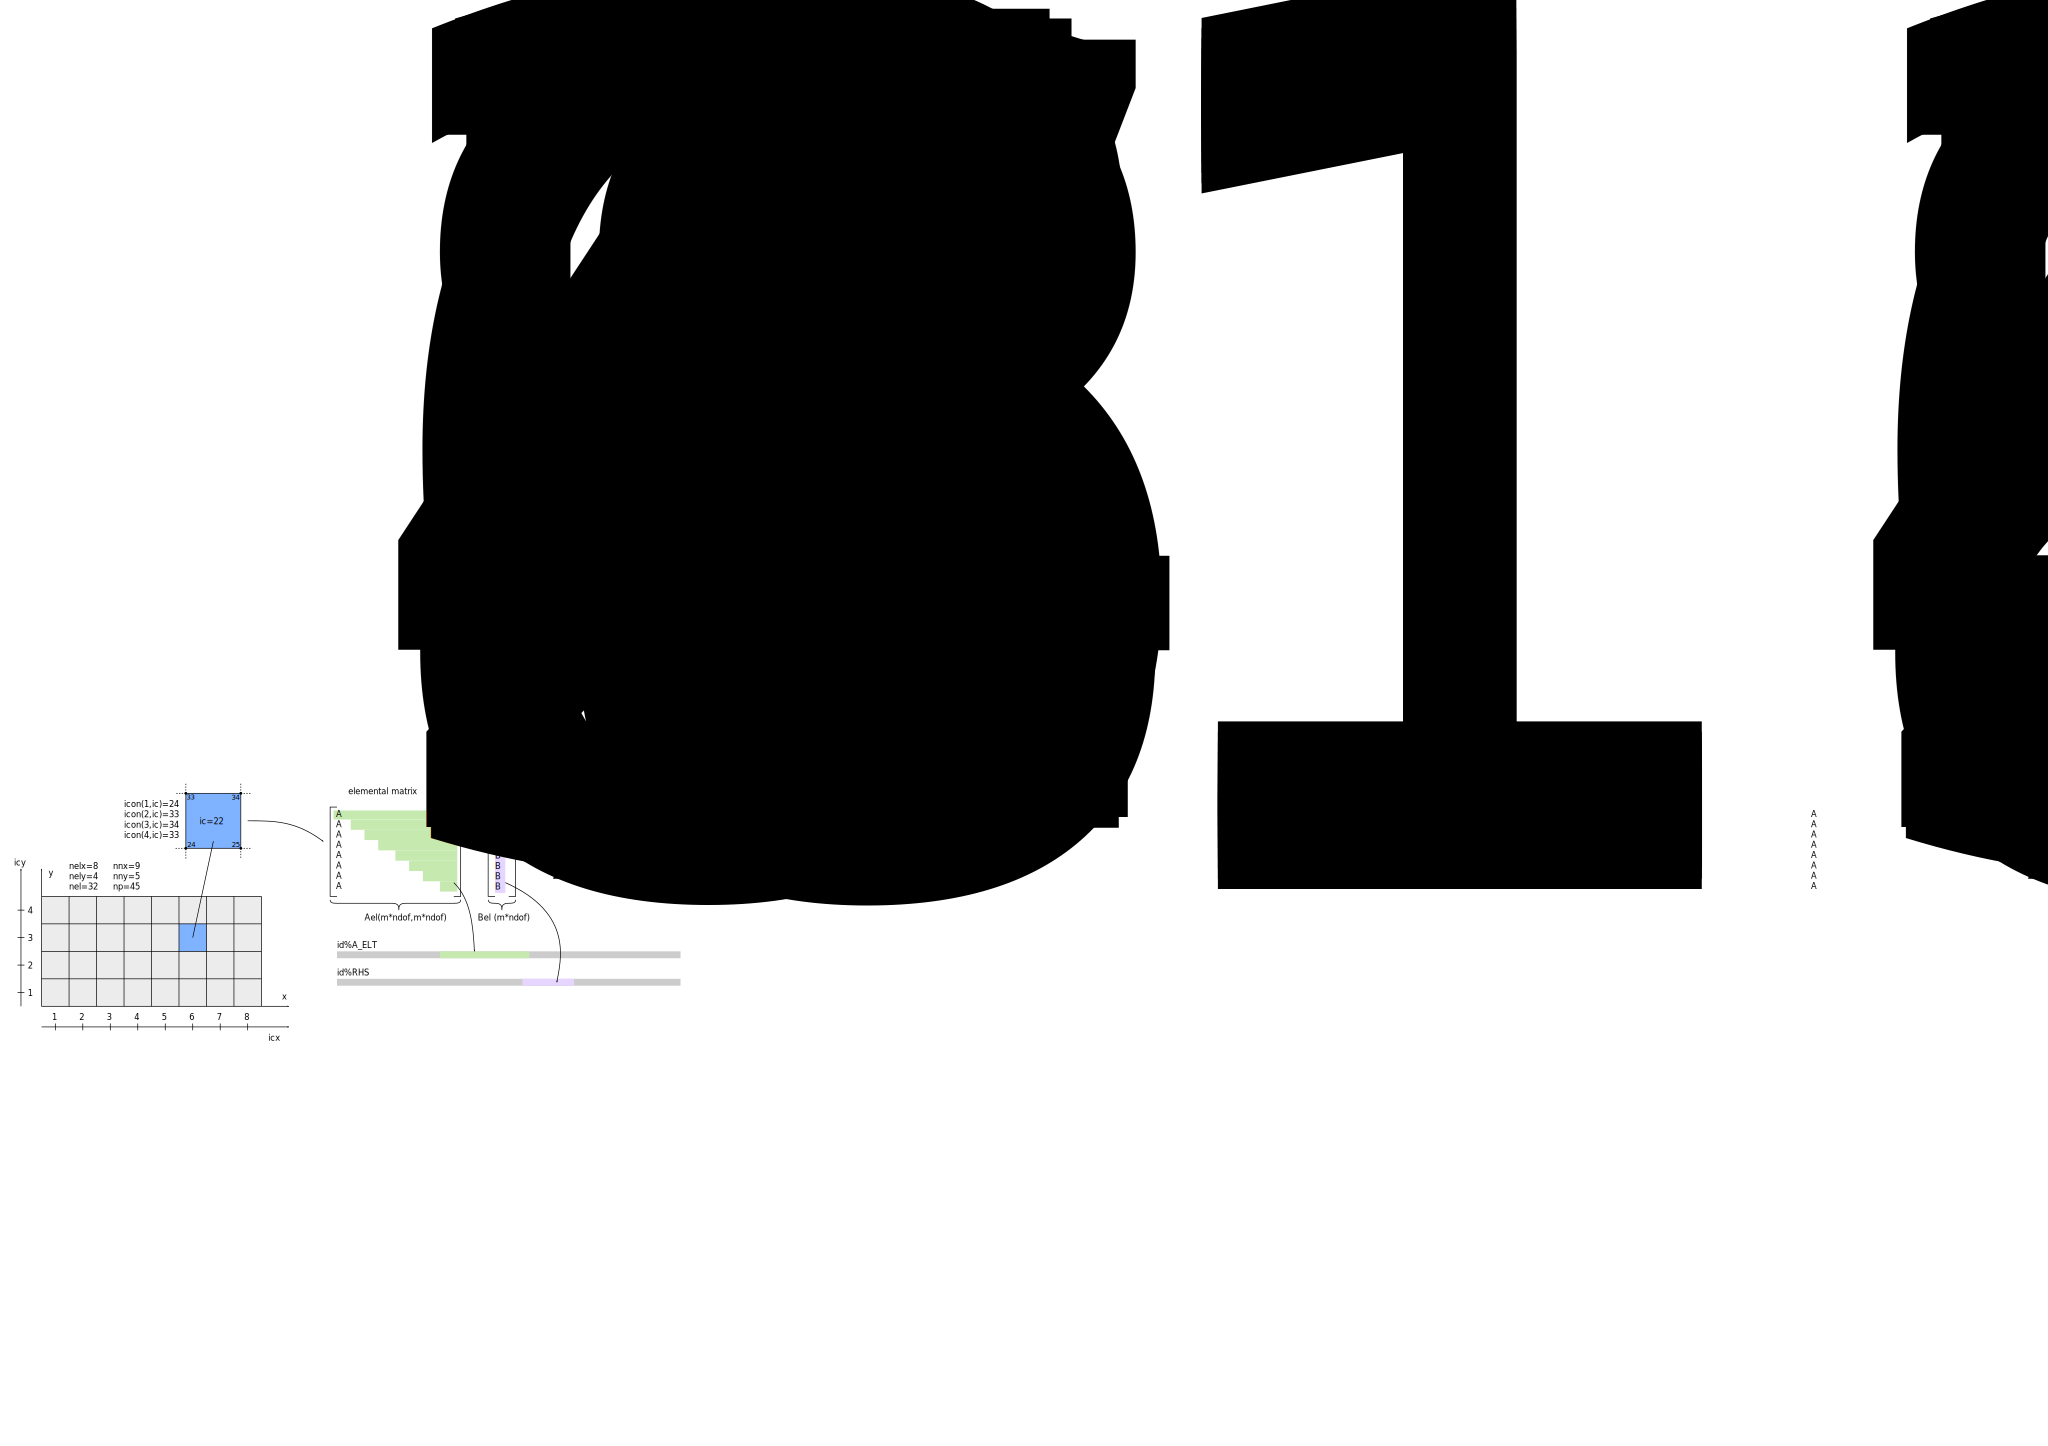
\includegraphics[width=4cm]{images/vtk/grid}
\includegraphics[width=4cm]{images/vtk/vel}
\includegraphics[width=4cm]{images/vtk/press}
\end{center}

In the same folder {\tt images/vtk} there is the python script 
{\pythonfile makevtu.py}\footnote{\url{https://raw.githubusercontent.com/cedrict/fieldstone/master/images/vtk/makevtu.py}} which produces 3 different vtu files. The first one {\sl solution1.vtu} is a similar to the one above: an \lstinline{nelx*nely} quadrilateral-based mesh in a unit square. 
The second one ({\sl solution2.vtu}) looks identical when opened in Paraview but it is rather different: each element is exported as its own sub-mesh, so that if the mesh counts nel elements the number of vertices is \lstinline{4*nel}, and not \lstinline{(nelx+1)(nely+1)}. As such this file is larger. The icon array is needed to write down the positions of the four vertices of each element but not to write down the connectivity since the first 4 points are making the 1st element, the next four points are making the second element, etc ...

\begin{lstlisting}
vtufile.write("<Points> \n")
vtufile.write("<DataArray type='Float32' NumberOfComponents='3' Format='ascii'> \n")
for iel in range(0,nel):
    if not flag[iel]:
       for k in range(0,m):
           vtufile.write("%10e %10e %10e \n" %(x[icon[k,iel]],y[icon[k,iel]],0.))
vtufile.write("</DataArray>\n")
vtufile.write("</Points> \n")
vtufile.write("<Cells>\n")
vtufile.write("<DataArray type='Int32' Name='connectivity' Format='ascii'> \n")
for iel in range (0,nel_left):
    vtufile.write("%d %d %d %d \n" %(iel*4,iel*4+1,iel*4+2,iel*4+3))
vtufile.write("</DataArray>\n")
...
vtufile.write("</Cells>\n")
\end{lstlisting}

This format is rather practical in the case of linear or higher order discontinuous fields. For example, in the case of the $Q_2\times P_{-1}$ element pair, the pressure is linear inside each element and discontinuous across element edges. One can then assign pressure values at the four vertices of each element.

Finally a third mesh {\sl solution3.vtu} is produced. It is based on the 2nd one, but since elements are now somewhat de-coupled, then one can export only a subset of the mesh. For instance one could not show elements which are two distorted, or below a certain line, or outside a certain volume, etc ... In {\pythonfile makevtu.py} all elements which center is inside a circle are flagged and will not be exported into the vtu file:
\begin{lstlisting}
for iel in range(0,nel):
    flag[iel]= (xc[iel]-0.333*Lx)**2+(yc[iel]-0.666*Ly)**2<0.234**2
nel_flagged=np.sum(flag)
nel_left=nel-nel_flagged
\end{lstlisting}

\begin{center}
\includegraphics[width=11cm]{images/vtk/mesh3}
\end{center}





